\setproblem{28119}

\begin{frame}[label=p1]{Traveling SCCC President(\prob)}

\tiny

\begin{block}{문제}
숭실대학교 컴퓨터학부 문제해결 소모임 SCCC의 회장인 찬솔이는 대회를 성공적으로 개최하기 위해 학교의 여러 건물에 들려 업무를 보고 있다.

숭실대학교의 캠퍼스는 
$1$번부터 
$N$번까지 번호가 붙어 있는 
$N$개의 건물과 서로 다른 두 건물을 연결하고 
$1$번부터 
$M$번까지 번호가 붙어 있는 
$M$개의 도로로 구성되어 있다. 
$i$번 도로는 
$u_i$번 건물과 
$v_i$번 건물을 연결하고, 이 도로를 이용해 한 쪽 건물에서 다른 쪽 건물로 이동하는데 
$w_i$분이 걸린다. 모든 건물은 도로를 통해 이어져 있다.

대회를 개최하기 위해서는 
$N$개의 건물에서 한 번씩 차례대로 회의를 진행해야 한다. 구체적으로, 회의를 진행해야 하는 건물의 순서 
$A_1,A_2,\cdots ,A_N$이 주어진다. 
$i$번째로 진행해야 하는 회의는 
$A_i$번 건물에서 진행되며, 모든 
$A_i$는 서로 다르다.

4차 산업혁명이 도래한 21세기에 매번 도로를 통해 이동하는 것은 비효율적이기 때문에, 찬솔이는 순간 이동 장치를 만들었다. 순간 이동 장치를 사용하면 지금까지 방문했던 건물 중 원하는 곳으로 순식간에 이동할 수 있다.

찬솔이는 
$S$번 건물에서 출발해서 
$N$개의 회의를 마친 다음 다시 
$S$번 건물로 돌아와야 한다. 시간이 부족한 찬솔이를 위해 
$N$개의 회의를 차례대로 모두 마치고 
$S$번 건물로 돌아오는데 걸리는 최소 시간을 구해주자.

\end{block}

\begin{block}{입력}
첫째 줄에 건물의 개수 
$N$, 도로의 개수 
$M$, 출발하는 건물의 번호 
$S$가 공백으로 구분되어 주어진다.

둘째 줄부터 
$M$개의 줄에 걸쳐, 
$i$번 도로가 연결하는 두 건물의 번호 
$u_i,v_i$와 도로를 통행하는 데 걸리는 시간 
$w_i$가 한 줄에 하나씩 공백으로 구분되어 주어진다.

$M+2$번째 줄에는 
$N$개의 정수 
$A_1,A_2,\cdots ,A_N$이 주어진다. 이는 
$i$번째 회의가 
$A_i$번 건물에서 진행됨을 의미한다.
\end{block}

\begin{block}{제한}
$2\leq N\leq 2\, 000; N-1\leq M\leq 5\, 000; 1\leq S\leq N; 1\leq w_i\leq 5\, 000$ 

모든 건물은 도로를 통해 이어져 있다.
\end{block}
\end{frame}


\begin{frame}{예제 입력 1}
\begin{center}
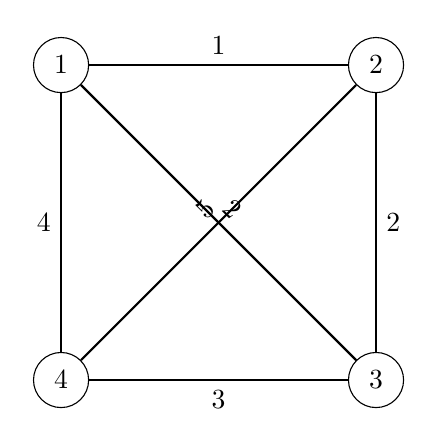
\begin{tikzpicture}[
    vertex/.style={circle, draw, minimum size=7mm},
    edge/.style={thick}
]

\node[vertex] (1) at (0,2) {1};
\node[vertex] (2) at (4,2) {2};
\node[vertex] (3) at (4,-2) {3};
\node[vertex] (4) at (0,-2) {4};

\draw[edge] (1) -- node[above] {1} (2);
\draw[edge] (2) -- node[right] {2} (3);
\draw[edge] (3) -- node[below] {3} (4);
\draw[edge] (4) -- node[left] {4} (1);
\draw[edge] (2) -- node[sloped, above] {5} (4);
\draw[edge] (1) -- node[sloped, above] {2} (3);

\end{tikzpicture}
\end{center}
\end{frame}

\begin{frame}{풀이(출처: 2023 SCON Editorial)}
\begin{itemize}
    \item 순간 이동을 하지 않고 직접 이동해야 하는 간선을 생각해 봅시다. 이 간선들은 연결 그래프를 이뤄야 하므로 정답은 MST의 가중치보다 크거나 같습니다.
    \item 이제 가중치가 MST와 동일한 해가 존재함을 보일 것입니다.
    \item MST를 만든 다음 1번 정점에서 시작하는 DFS를 수행합시다.
    \item 방문하지 않은 정점으로 이동할 때 직접 이동하고 다시 돌아올 때 순간 이동을 하면 정확히 MST와 동일한 가중치로 모든 정점을 방문할 수 있습니다.
    \item 모든 정점을 한 번씩 방문한 이후에는 순간이동만을 사용해 시간의 소요 없이 모든 회의를 진행할 수 있습니다.
\end{itemize}
\end{frame}

\begin{frame}[fragile, allowframebreaks]{원찬혁 소스 코드}
\inputminted{java}{../src/\prob/Chanhyeok/Main.java}
\end{frame}

\begin{frame}[fragile, allowframebreaks]{손현준 소스 코드}
\inputminted{java}{../src/\prob/hyunjun/P24116.java}
\end{frame}

\begin{frame}[fragile, allowframebreaks]{김지훈 소스 코드}
\inputminted{java}{../src/\prob/Jihoon/BOJ_28119.java}
\end{frame}

\begin{frame}[fragile, allowframebreaks]{김준형 소스 코드}
\inputminted{java}{../src/\prob/junhyeong/Main.java}
\end{frame}

\begin{frame}[fragile, allowframebreaks]{임건애 소스 코드}
\inputminted{java}{../src/\prob/keonae/b28119.java}
\end{frame}

\begin{frame}[fragile, allowframebreaks]{서민종 소스 코드}
\inputminted{java}{../src/\prob/Minjong/Main.java}
\end{frame}

\begin{frame}[fragile, allowframebreaks]{정의찬 소스 코드}
\inputminted{java}{../src/\prob/Uichan/"Traveling SCCC President".java}
\end{frame}

